% (c) Christoph Lange 2007
\documentclass{llncs}

% Draft?
\newif\ifdraft
\drafttrue
%\draftfalse

% \usepackage[english]{babel}
\usepackage[T1]{fontenc}
\usepackage[utf8]{inputenc}
\usepackage{lmodern}
\usepackage{textcomp}

\ifdraft
\usepackage[show]{ed}
%\usepackage{pdfsync}
\else
\usepackage[hide]{ed}
\usepackage{microtype}
\fi


% \usepackage{a4wide}
\usepackage{amsmath}
\usepackage{amsfonts}
\usepackage{amstext}
% \usepackage{array}
% \usepackage{graphicx}
% \usepackage{ifthen}
\usepackage{listings}
% \usepackage{lstpatch}
% \usepackage{lstomdoc}
% \usepackage{makeidx}
% \usepackage{scrpage2}
% \usepackage[binary,squaren]{SIunits}
% \usepackage{supertabular}
% \usepackage{tabularx}
% \usepackage{thm2e}
% \usepackage[normalem]{ulem}
\usepackage{wrapfig}
% \usepackage[svgnames]{xcolor}

\usepackage{tikz}

% % Symbol fonts
% \let\RealRightarrow=\Rightarrow
% \usepackage{marvosym}
% \renewcommand{\Rightarrow}{\RealRightarrow}
% \usepackage{wasysym}

% KWARC packages
\usepackage{acronyms,myindex,semantic-markup}
% \let\Realstex=\stex
% \usepackage{paths}
% \renewcommand{\stex}{\Realstex}

% ... and adjustments
\def\omdocni{{\sc OMDoc}} % non-indexed OMDoc
\def\swimni{{\sc SWiM}} % non-indexed SWiM

\hyphenation{name-space}
\hyphenation{Me-dia-Wi-ki}

% Local abbreviations
% \def\abSMW{\product{Semantic MediaWiki}}

% TikZ setup
\usetikzlibrary{arrows}
\tikzstyle{default}=[font=\sffamily,>=triangle 60]
\tikzstyle concept=[font=\sffamily\bfseries,draw,minimum height=3.5ex,rounded corners]

% % Page styles
% \pagestyle{scrheadings}
% \clearscrheadfoot
% \ohead{\headmark}
% \ofoot[\pagemark]{\pagemark}
% \setheadsepline{0.3pt}[\color{gray}]
% \setkomafont{pagehead}{\normalfont\small\sffamily\slshape}
% \setkomafont{pagenumber}{\normalfont\small\sffamily\slshape}
%
% % Listing styles
\lstset{float=htb,columns=flexible,frame=lines,basicstyle=\footnotesize\ttfamily,
        showstringspaces=false,basewidth=.5em}
%
% % Array setup
% \newcolumntype{v}[1]{>{\raggedright\arraybackslash\hspace{0pt}}p{#1}}

\def\thetitle{Flyspeck in a Semantic Wiki -- Collaborating on a Huge Mathematical Proof}

% load this last
% \definecolor{NavyBlue}{cmyk}{0.94,0.54,0,0.3}
% \usepackage[pdftex,pdfstartview=FitV,plainpages=false,pdfpagelabels,colorlinks=true,linkcolor=NavyBlue,citecolor=NavyBlue,urlcolor=NavyBlue,hypertexnames=true]{hyperref}
% \hypersetup{
%     pdfauthor = {Christoph Lange},
%     pdftitle = {\thetitle},
%     pdfkeywords = {Semantic Wiki OMDoc Ontology Services Science Mathematical
% Knowledge Management Mathematics}
% }
\usepackage{url}

% \hypersetup{bookmarksdepth=4}

\title{\thetitle}
\author{Christoph Lange\inst{1} \and Sean McLaughlin\inst{2} \and Florian Rabe\inst{3}}
\institute{Computer Science, Jacobs University Bremen\thanks{formerly
International University Bremen}, \email{\{ch.lange,f.rabe\}@jacobs-university.de} \and
School of Computer Science, Carnegie Mellon University, Pittsburgh, \email{Sean's e-mail}}

\begin{document}

\maketitle

\ednote{To do: make the title a little bit less boring}

\begin{abstract}
  Semantic wikis have been successfully applied to many problems in knowledge management
  and collaborative authoring.  That makes them appropriate for e-science, and
  for mathematical knowledge management in particular.  Building on the OMDoc semantic markup
  language, we have developed an ontology for mathematical knowledge and a semantic wiki
  based thereon, and we are now evaluating these technologies in concrete application
  scenarios.
  
  The purpose of the Flyspeck project is to develop a formally verifiable proof of
  Kepler's century-old conjecture about packing balls in three-dimensional
  space.\ednote{@Sean: Emphasize that this is a HUGE proof.}  Flyspeck is estimated to
  take more than twenty person-years\ednote{@Sean: right? --CL}, which makes it naturally
  applicable to a ``crowdsourcing'' approach.

  In this paper we evaluate the applicability of semantic wikis to the Flyspeck use case:
  With lessons learned from a rapid-prototyping study with Semantic MediaWiki, we
  establish a roadmap how to improve our own, mathematics-specific semantic wiki SWiM to
  meet the needs of the Flyspeck collaborators even better.
\end{abstract}

@Sean, I inserted this auto-generated message. Have you ever written something together
with Florian? Then you probably know our ednote macros. Anyway, this is just FYI, and
after having read it, you may delete it :-) --Christoph
\hrule
\edexplanation
\hrule

\section{A Semantic Wiki for e-Science}

\begin{wrapfigure}{r}{5.5cm}
  \centering
  \vspace{-.5cm}
  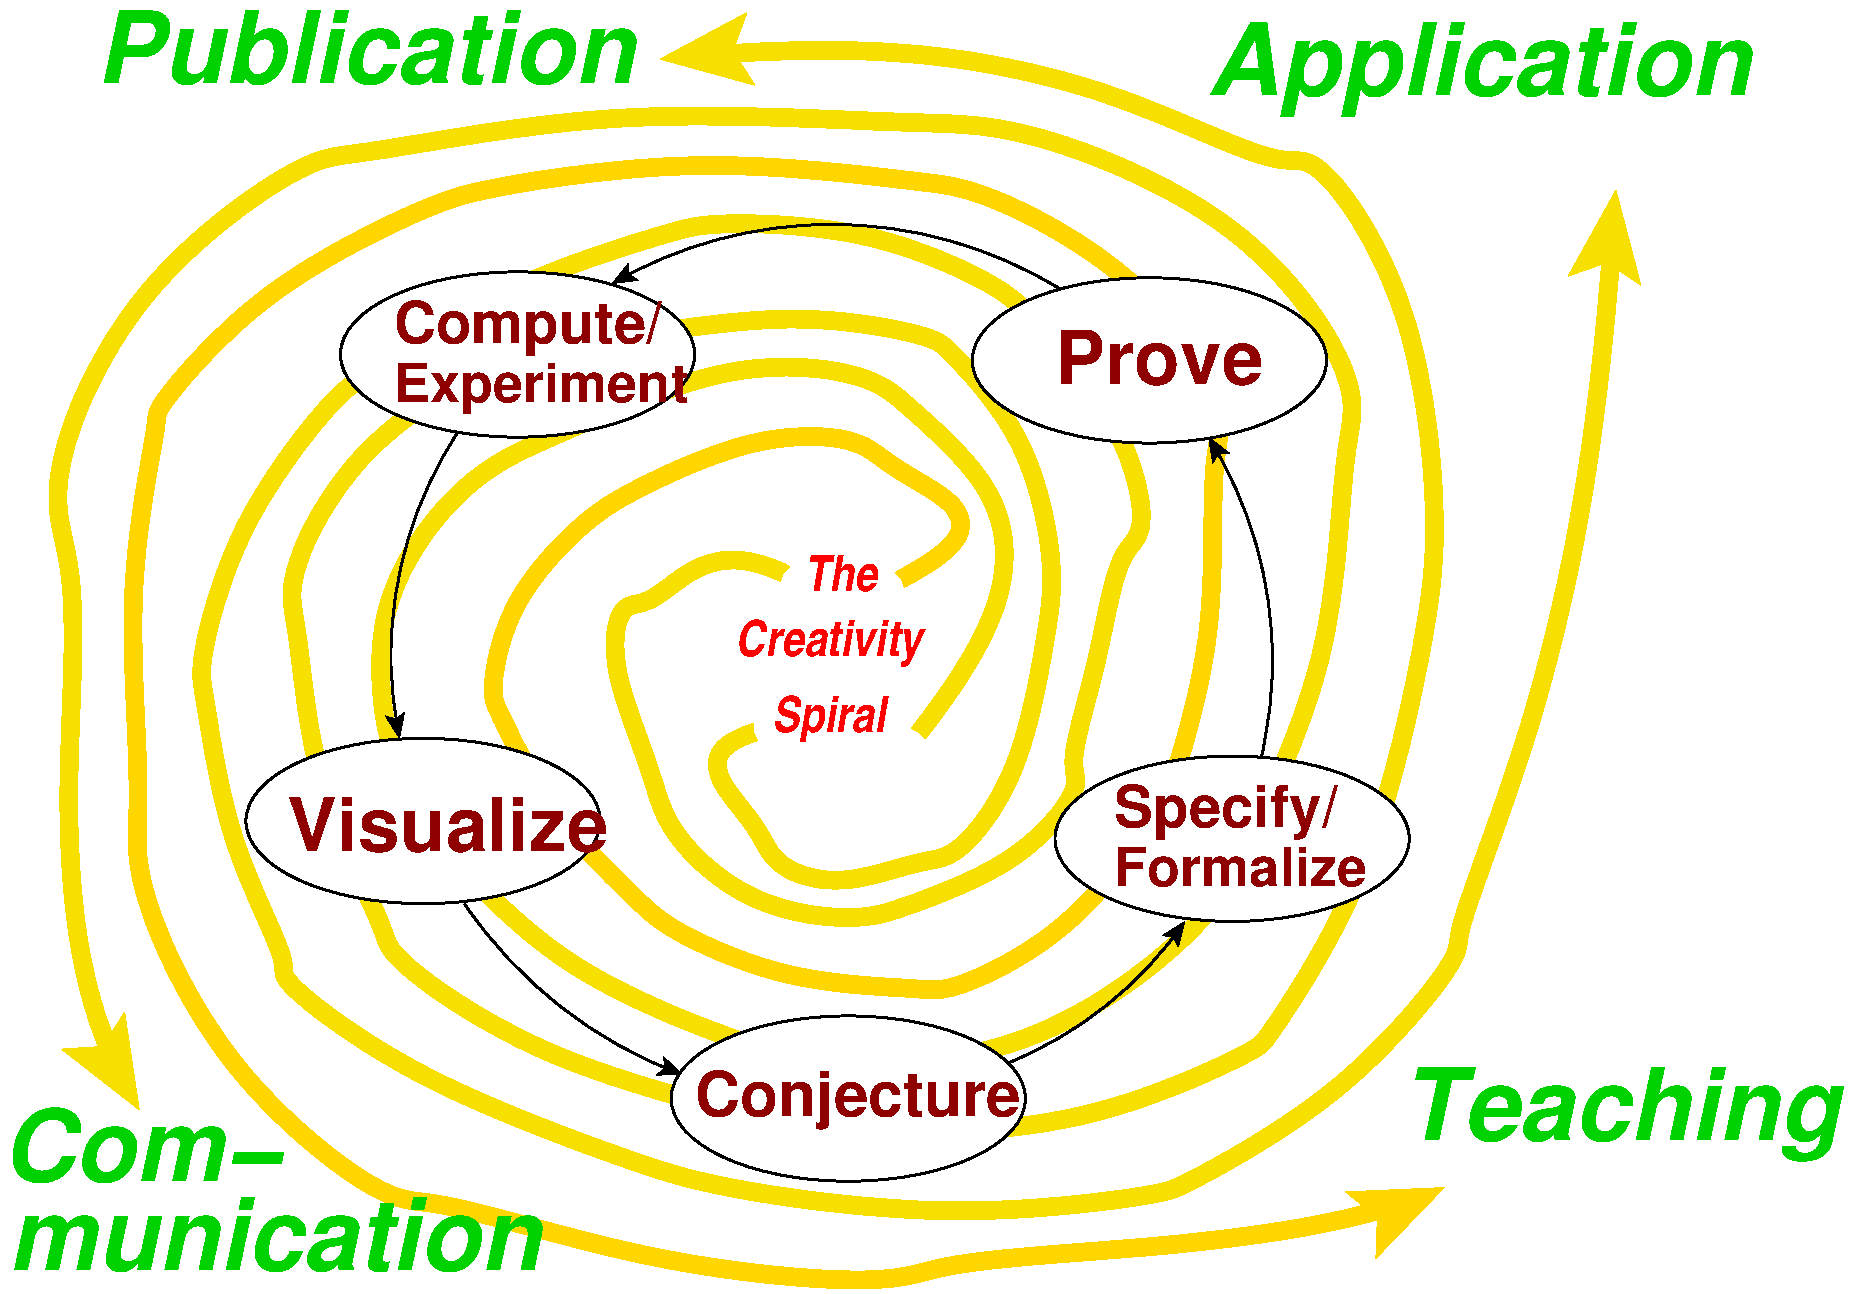
\includegraphics[width=5cm]{creativity-spiral}
  \vspace{-.5cm}
  \caption{The Math/Science Creativity Spiral (after Buchberger, 1995)}
  \label{fig:creativity-spiral}
\end{wrapfigure}
A great deal of scientific work consists of collaboratively authoring documents --- taking
down first hypotheses, commenting on results of experiments or project steps, as well as
structuring, annotating, and re-organizing existing items of knowledge.  Obviously, tools
that \emph{understand} the knowledge contained in scientific documents are desirable for
editing them.  One approach towards this is writing scientific documents in a semantic
markup language with an editor that knows the structures available in this language.

Besides generic approaches like SALT~\cite{Groza:SALT07}, semantic markup has been most
deeply investigated in the specific domain of mathematics with its complex and explicit
structures\ednote{reword}, resulting in languages like MathML, OpenMath, and
OMDoc~\cite{Kohlhase:omdoc1.2}.  OMDoc is a language that employs Content
MathML\footnote{MathML comes in two flavors: Presentation MathML expresses the way a
  formula is rendered, whereas Content MathML models its logical structure.  Formal
  mathematical software like a Computer Algebra System would export formulae in Content
  MathML, but for publishing, they would be converted to Presentation MathML.} or OpenMath
for structurally representing mathematical \emph{objects} (symbols, numbers, equations,
etc.) and adds two layers on top of that: Objects or informal text can be annotated as
mathematical \emph{statements} (symbol declarations, definitions, axioms, theorems,
proofs, examples, etc.), and collections of interrelated statements are grouped into
\emph{theories}.

With SWiM, a semantic wiki for mathematical knowledge management (see
section~\ref{sec:swim}, we have investigated collaborative editing of OMDoc documents.  It
has turned out that a wiki is a suitable tool for supporting the incremental workflow of
scientific writing.  But wikis have not only shown to be appropriate for \emph{writing},
but also for project management, e.\,g.\ in corporate settings~\cite{leuf01:wikiway}.
Thus, we are interested in applying our technologies to scientific knowledge engineering
projects.  The Flyspeck project (see section~\ref{sec:flyspeck}) was particularly
appealing as a use case: It involves both highly formal and semi-formal mathematical
knowledge, as well as informal text, and it was found te be suitable for ``crowdsourcing''
and supporting the project organization by social software.  This is suggested by its
large extent and the required manpower.  We anticipate that the three conditions for
successful peer production stated by Tapscott and Williams~\cite{wikinomics} will hold or
can be satisfied by software support: The object of production is information, which keeps
the cost of participation low, tasks (i.\,e.\ lemmas to be proven) can mostly be broken
down into small, independent pieces, and the cost of integrating the individual
contributions is low.

\section{The Flyspeck Project (Sean)}
\label{sec:flyspeck}

Kepler conjecture (probably with a nice drawing?) -- one of the greatest problems of
mankind

Hales' original proof -- its enormous size (mention number of areas of mathematics
covered) and why it's not been accepted

Flyspeck project\cite{hales:DSP:2006:432}

So far on Google code (see section~\ref{sec:req})

Idea to get the community involved -- give them a wiki (leading the way to Christoph's
part: As we want to exploit certain structural properties of the proof, we'd like to have
a \emph{semantic} wiki that is capable of handling them)

\begin{enumerate}
\item make the whole extent of the proof graspable
\item make the workflows manageable
\item later maybe support proof development/proof validation right in the wiki?
\end{enumerate}

\begin{todo}{@Christoph}
  Motivate this with the principles of wikinomics \url{http://www.wikinomics.com}: If a
  smart but poor boy in Africa with his OLPC accesses our homepage\ldots
\end{todo}

\section{State of the Art}
\label{sec:sota}

\subsection{Mathematical Knowledge Management (Florian/Christoph)}
\label{sec:mkm}

\begin{todo}{@Christoph: Look this up in the literature}
Project before the age of computer-supported MKM: classification of the final groups
\end{todo}

Theorem provers and their libraries (all with a central repository and a repository
viewer): Mizar, Coq, PVS

formal and informal aspects of mathematical knowledge, content markup; OMDoc covering both
formal and informal aspects.  Actually, we're now interested in semi-formal
knowledge:
\begin{itemize}
\item documenting formal knowledge (the proof, or the theorems to be proved, resp.)
\item from informal ideas (how to prove sth.) to formal proofs
\end{itemize}

\subsection{Wikis for Mathematics (Christoph)}
\label{sec:math-wiki}

\subsubsection{Semantic Wikis}
\label{sec:semwiki}

Semantic wikis~\cite{semwiki06} are wikis enhanced by semantic annotations.  Although many
ways of semantically enhancing wikis have been investigated, a modelling approach prevails
where one resource (in the RDF sense) --- e.\,g.\ one mathematical theorem --- is
represented by one wiki page and relations between resources by links between pages.  Both
pages and links can be typed with terms from
ontologies~\cite{OrDeMoVoHa06:annotation-navigation-semwiki}, which are either preloaded
into the wiki or modelled ad-hoc~\cite{KrSchVr:semwiki-reasoning07}.  Semantic wikis
commonly offer enhanced navigation capabilities by displaying a summary of all typed
links, grouped by type, with each page.  Most of them allow to search for pages by type or
by them being subject or object of any RDF triple (= typed link), while it depends on the
reasoner used by the wiki whether only explicit RDF triples or also inferred ones are
considered~\cite{KrSchVr:semwiki-reasoning07}.  Such queries can usually be executed
interactively via a special search form, or in an automated way as \emph{inline} queries
embedded into the content of a page.

\subsubsection{Informal Knowledge Collections}
\label{sec:math-knowledge-collections}

Current collaborative projects for managing \emph{informal} mathematical knowledge range
from comprehensive encyclopediæ like the mathematical sections of \product{Wikipedia} or
the courseware repository and content management system \product{Connexions} to projects
specially focused on mathematics like \product{PlanetMath}\footnote{See
  \url{http://www.wikipedia.org}, \url{http://cnx.org} or \url{http://www.planetmath.org},
  respectively.}, which is powered by a highly customized wiki-like system.  The pages in
these systems are categorized and searchable in full-text, with additional metadata
records in the case of \product{PlanetMath}.  Neither of these systems is a
\emph{semantic} wiki, and thus they fail to solve the following two problems, which are
essential for MKM:

\begin{enumerate}
\item\label{item:formula-search-usecase} In \product{Wikipedia} and \product{PlanetMath},
  formulæ are given in presentation-oriented {\LaTeX}.  Imagine a wiki page about the
  Pythagorean Theorem, stated as $a^2 + b^2 = c^2$, and a user searching for the
  equivalent formula $x^2 + y^2 = z^2$ (or even $c=\sqrt{a^2+b^2}$!) --- The system would
  not find the theorem.
\item Neither could ``all theorems about triangles for which a
  proof exists'' be searched for, as the link from a proof to the theorem it proves is not
  typed.
\end{enumerate}

\product{Connexions}, on the other hand, could in principle cope with these two problems,
but in practice it does not: Formulæ are written in the content-oriented sublanguage of
{\mathml}~\cite{CarlisleEd:MathML07}, and the CNXML markup language used for larger
structures allows for annotating texts as mathematical statements like lemmas, but this
structural information is not yet \emph{used} by the system.  Moreover, none of the
systems mentioned so far supports an easy navigation from the occurrence of a mathematical
symbol in a formula to the declaration or definition of this symbol, if it is defined in
some other place of the wiki; instead, the author has to provide links he considers
relevant in the text surrounding the formula.

\subsubsection{Domain-Specific Semantics}
\label{sec:domain-semantics}

Note that general-purpose semantic wikis do not support the above-mentioned use case
(\ref{item:formula-search-usecase}) either, as they neither have a sufficient notion of
equality nor understand mathematical content markup.  If we assume ``semantic'' not just
to mean RDF or description logics, but any kind of (higher-order) logic required for
specific domains\ednote{@Florian: This is quite superficial, can we write it in a more
  sophisticated way?} and employ domain-specific ways of knowledge representation we can
imagine semantic wikis specifically supporting mathematics.  For use case
(\ref{item:formula-search-usecase}), we could have the wiki pages crawled by a formula
search engine like MathWebSearch~\cite{KohSuc:asemf06}, which applies substitution tree
indexing to mathematical formulae.  Even more formal approaches integrate automated
theorem provers into wikis.  Two of these systems are discussed in
section~\ref{sec:wiki-pa}.

\section{Supporting Flyspeck in a Semantic Wiki (Christoph)}

Starting from requirements how collaborating on formalizing the Kepler proof should be
supported, we have evaluated the applicability of two concrete semantic wikis to Flyspeck
in order to see what possibilities this technology can offer for the project:  our own
semantic wiki SWiM, and a rapid prototype developed on top of Semantic MediaWiki.  Based on the
results of this pre-study, we establish a roadmap for tailoring SWiM to specifically meet
the needs of the Flyspeck collaborators.

\subsection{Workflow Requirements (Christoph, Sean)}
\label{sec:req}

So far, the Flyspeck project has had two\ednote{@Sean, fix the number!} core members who
collaborated via Google Code~\cite{flyspeck:web}.  While the services offered by Google
Code (a Subversion repository, a mailing list, and others) were found to be sufficient for
the core development team, we were not satisfied with the wiki integrated into the Google
Code web interface.  Lacking support for mathematical formulae, it would not even allow
for presenting the theorems and lemmas to be formally proved in a human-readable fashion.
Secondly, besides untyped links and adding labels to pages it does not offer any further
\emph{structuring} support, which we found essential for browsing and querying Flyspeck's
large knowledge collection.

In this early phase of ``crowdsourcing'' Flyspeck, the focus is not yet on developing and
checking formal proofs collaboratively, but on making its extent and structure
comprehensible and on communicating where work needs to be done.  For this the outline of
the whole proof from the book\ednote{@Sean, I guess I should assume that you introduce the
  book in the Flyspeck intro. --CL} needs to be represented in the wiki, where the
mathematical statements (including definitions, lemmas, and theorems) are available in a
human-readable way (with formulae in \LaTeX\ or presentational MathML) as well as a
machine-readable presentation suitable for downloading into a theorem prover.  In order to
obtain a well-structured network of knowledge items, each mathematical statement should be
presented on one wiki page, which shows its human-readable representation from the book,
offers additional space for annotation, and allows for downloading a formal
representation.  We considered the following kinds of annotations desirable:

\begin{description}
\item[Categorization by topic:] In the beginning, one would mirror the narrative structure
  of the book (e.\,g.\ ``ball'' being a subsection of ``primitive volumes'', which in turn
  is a section of the chapter ``volume calculations'').  Standardized ways of classifying
  mathematical topics, such as the Mathematical Subject Classification
  (MSC)\ednote{reference}, could be added later.
\item[Project-organization metadata] such as the information whether a lemma has already
  been proven formally, or in what theorem proving language there are proof objects
  available.\ednote{@Sean: more?}
\item[Dependency links:] These can be links from individual symbols in mathematical
  formulae to the place where they are declared, or from any page $p$ to other pages
  containing knowledge that is required for understanding $p$ --- either pages in the same
  wiki, or external resources like PlanetMath or Wikipedia articles.
\item[Discussion posts] should be strongly tied to the topic being discussed, and they
  should be classified into categories like question, answer, explanation,
  etc.
\end{description}

To the visitor and potential collaborator, an impression of the extent and structure of
the project --- its enourmous size and its specialization into diverse fields of
mathematics --- must be given, as well as tools for browsing and querying the knowledge.
The topical structure as well as the dependencies must be browsable via links.  Not only
should it be possible to query knowledge items by their annotations, but important query
results must also be available as dynamically generated lists.  Examples for queries are:

\begin{enumerate}
\item\label{item:proven-lemma} ``Which lemmas about composite regions have not been
  formally proven so far?''
\item ``What do I need to read in order to understand Jordan's curve
  theorem?''\ednote{internal dependency graph, tutorial, planetmath}
\item ``What lemmas are difficult to prove?''
  \begin{enumerate}
  \item \ldots in the sense that many invalid proofs have already been submitted
  \item\label{item:question-count} \ldots in the sense that many people have asked
    questions in the related discussion
  \end{enumerate}
\item \ldots\ednote{@Christoph: Check Matthias' BSc thesis for further ideas. --CL}
\end{enumerate}

A volunteer who is willing to work out and contribute a formal proof for some lemma should
be able to download a self-contained formal representation of this lemma and everything it
depends on.  Different notions of dependency could make sense: The strongest one is that a
lemma depends on the declarations and definitions of all symbols it uses and on the
transitive closure of all symbols used by the latter---i.\,e.\ the minimum set of
knowledge required to \emph{understand} the respective lemma.  This would, however,
require a collaborator to develop his new proof from scratch.  We anticipate that it will
be more desirable for a user to download other, previously proven
lemmas\ednote{@Sean/Florian: and their proofs? Does one also need proof objects for that?}
as well and treat them like axioms.  Assuming that the Flyspeck book\ednote{rename} is
written in a reasonable order, this would be all lemmas \emph{before} the current one, in
the narrative order of the book.  But it should still be possible to download \emph{all}
theorems, as a creative proof might involve lemmas one would not think of
first.\ednote{@Florian: Do we want to convert between theorem proving languages?  Is this
  feasible with OMDoc?}.

For the integration of the contributed proofs, we currently envisage that a small group of
maintainers will integrate submitted formal proofs into one central ``master'' proof
script outside of the wiki and have this script checked semi-automatically.  Metadata
\emph{about} the progress of the proof, e.\,g.\ whether a submission by a certain user was
valid, and a human-readable outline of the proof\ednote{@Sean: This as well?  Is it
  technically possible to explain a machine proof to a human.} will be added to the wiki.
In a later phase, it has to be investigated whether formal proofs can also be
collaboratively developed and validated in the wiki (cf.\ section~\ref{sec:wiki-pa}).

\newcommand{\wikipage}[5]{\node[draw,text width=5cm,font=\tiny\sffamily] (#1) at #2 {
    {\footnotesize\bfseries #3}\\
    #4
    ~\\[1em]
    [Download Isabelle representation]\\
    #5
  };}
\begin{figure}
  \centering
  \begin{tikzpicture}[set style={{default}+=[scale=1.5,font=\sffamily]},default,xscale=.8]
    \wikipage{lemma}{(0,0)}{Lemma 1.3}{The cosine is an even function.  The sine is an odd function.\\
      $\cos(-x)=\cos(x),\qquad\sin(-x)=-\sin(x)$}{Page type: Lemma\\
      Topic: Trigonometry\\
      Proven: no (3 unsuccessful attempts)}
    \wikipage{cos}{(6,0)}{Cosine}{$cos\colon\mathbb{R}\to\mathbb{R},x\mapsto\ldots$}{
      Page type: Definition\\
      Topic: Trigonometry
    }
    \wikipage{todo}{(0,3)}{To do}{Unproven lemmas:
      \begin{itemize}
      \item Lemma 1.3
      \item \ldots
      \end{itemize}
    }{
      Page type: Overview
    }
    \draw[->] (lemma) -- node[above] {usesSymbol} (cos);
    \draw[->] (todo) -- node[left] {references} (lemma);
  \end{tikzpicture}
  \caption{Page structure}
  \label{fig:pagestructure}
\end{figure}

In the following two sections, we evaluate SWiM 0.2 and a prototype based on Semantic
MediaWiki for their applicability to Flyspeck with regard to their support for
annotations, browsing, and querying.  For the case study, we had the {\TeX} sources of the
Flyspeck book and a Twelf formalization of the first chapter (Trigonometry) at our
disposal.\ednote{@Sean/Florian: One/two sentences about Twelf!}  Currently we are
investigating whether Twelf is actually appropriate for formalizing Flyspeck.  We are also
investigating Isabelle, but we consider the design of the wiki support to be largely
independent of that decision.  After ???\ednote{@Sean: insert number} years, we consider
the basic narrative structure of the book a sufficiently stable for modeling the structure
of the wiki after it.  During the formalization of the knowledge, we anticipate that
mainly its axiomatic parts (i.\,e.\ the way concepts are defined) will undergo major
refactoring in order to facilitate the actual development of the proofs, as certain areas
of mathematics the Kepler proof heavily relies on, such as geometry, are underrepresented
in the existing formal mathematical libraries of theorem provers\ednote{@Sean: this is in
  a nutshell what you once told me about this; is it sufficient?}.  Additional refactoring
support by the wiki would thus be of advantage.

Secondly, we have not yet committed to a definitive workflow for formalizing the book.
Given the size of the book, which is much smaller than the size of the final
proofs\ednote{@Sean: right?}, the current Flyspeck core team may be able to create formal
representations of the symbol declarations, definitions, and lemmas manually and upload
them to the wiki.  On the other hand, wikis support a workflow where different groups of
authors, such as domain experts or proof-readers, collaborate in formalizing knowledge
step by step.  This potential could also be unleashed for Flyspeck.

\subsection{SWiM 0.2}
\label{sec:swim}

SWiM is a semantic wiki for mathematical knowledge management.  Based on the
general-purpose semantic wiki IkeWiki~\cite{KrSchVr:semwiki-reasoning07}, it adds support
for browsing, editing, rendering, importing and exporting mathematical documents written
in OMDoc.  The semantics of mathematical knowledge is mainly captured in a \emph{document
  ontology}: Whenever a wiki page containing OMDoc fragments is stored, its type and its
(typed) relations to other items of mathematical knowledge in the wiki are extracted from
the OMDoc XML markup and explicitly represented as RDF triples in terms of the OMDoc
document ontology~\cite{OMDocDocOnto:web}.  This ontology models those aspects of the
three layers of mathematical knowledge supported by OMDoc to the extent supported by the
expressivity of OWL-DL.  Modeling all modules of the OMDoc specification in this ontology
is work in progress; so far, most mathematical statements as well as key aspects of
theories have been implemented.  Relevant classes for Flyspeck would be
\textit{Lemma}/\textit{Theorem}/\textit{Corollary}/\ldots (all being subclasses of
\textit{Assertion}), \textit{Proof}, \textit{Symbol} (a symbol declaration),
\textit{Definition}, and the properties \textit{Proof--proves--Assertion} and
\textit{Symbol--hasDefinition--Definition}.  Dependencies can partly be inferred by a DL
reasoner, but for a complete support of OMDoc's notion of dependency, an OMDoc-specific
calculus will have to be applied, which is currently in development.

\begin{figure}
  \centering
  \begin{tikzpicture}[set style={{default}+=[scale=.47,font=\normalsize\sffamily]},default]
    \tikzstyle{every path}=[font=\small\sffamily];
    \node[concept] (s) at (0,0) {\itshape Statement};
    \node[concept] (d) at (-7.5,-3) {Definition};
    \node[concept] (y) at (-2.5,-3) {Symbol};
    \node[concept] (a) at (+2.5,-3) {Assertion};
    \node[concept] (p) at (+7.5,-3) {Proof};

    \node[concept] (l) at (-1.5,-6) {Lemma};
    \node[concept] (c) at (+2.5,-6) {Corollary};
    \node[concept] (t) at (+6.5,-6) {Theorem};

    \draw[-open triangle 60] (y) -- (s);
    \draw[-open triangle 60] (d) -- (s);
    \draw[-open triangle 60] (a) -- (s);
    \draw[-open triangle 60] (p) -- node[right=1ex] {$\sqsubseteq$} (s);

    \draw[-open triangle 60] (l) -- (a);
    \draw[-open triangle 60] (c) -- (a);
    \draw[-open triangle 60] (t) -- (a);

    \draw[->] (d) -- node[below] {uses} (y);
    \draw[->] (a) -- node[below] {uses} (y);
    \draw[->] (p) -- node[below] {proves} (a);

    \draw[->] (s.0) .. controls +(0:2cm) and +(60:2cm)
    .. node[right=1pt,text width=2cm,text centered] (dep)
    {\itshape depends on} (s.60);

    \draw[->] (y.-120) .. controls +(-120:1cm) and +(-60:1cm) .. node[below] {hasDefinition} (d.-60);
  \end{tikzpicture}
  \caption{A relevant subset of the OMDoc document ontology}
  \label{fig:doconto}
\end{figure}

In the current version 0.2 of SWiM, the browsing of mathematical documents is powered by
the document ontology: Whenever RDF triples having the current page as subject or object
are available, most of them using terms from the OMDoc document ontology if the current
page is a mathematical document, they are displayed as navigation links (see
figure~\ref{fig:swim-lemma}).  Adding more ontology-powered services, particularly ones
that facilitate editing documents, is planned for version
0.3~\cite{swim-roadmap,Lange:SWiMSciColl07}.  Documents are presented as XHTML+MathML,
generated by the \textit{mmlkit} renderer~\cite{mmlkit:web}, with mathematical symbols
linked to their declarations.

\begin{figure}
  \centering
  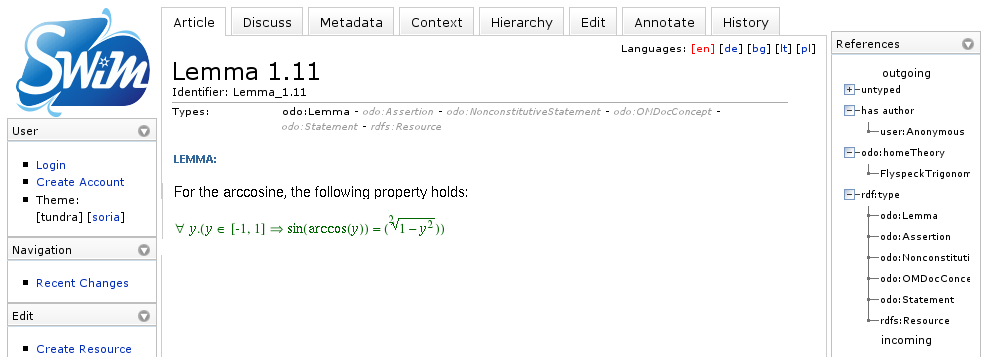
\includegraphics[width=.7\textwidth]{swim-lemma}
  \caption{A Flyspeck lemma in SWiM}
  \label{fig:swim-lemma}
\end{figure}

We manually recreated one Flyspeck lemma in SWiM and judged about the further annotation
capabilities from our previous experience with implementing SWiM and modeling other
document collections (as the OpenMath content dictionaries) in the system.\ednote{This is
  honest and really sufficient IMHO, but maybe sounds a bit weak -- what do you think?
  --CL} For testing a larger subset of Flyspeck, it would, however, have been possible to
convert the Twelf master source to OMDoc with our already existing converter, and to
import the generated OMDoc documents into SWiM using the built-in import functionality.
OMDoc would offer excellent support for the alternative workflow of stepwise formalization
as well~\cite[chap.\ 4]{Kohlhase:omdoc1.2}.  One could either start with converting the
Flyspeck book from {\LaTeX} to HTML with Presentation MathML and step by step formalize
the presentation markup into content markup, or one could start the formalization on the
{\TeX} side, using s\TeX{}, a content-oriented {\TeX} notation for OMDoc which can then be
converted to OMDoc~\cite{Kohlhase:albwo06}.

We found SWiM to be suitable for making Flyspeck browsable, as it supports breaking down
mathematical knowledge to the statement level and recognizes all required link types.  As
every SWiM page has an associated discussion page and discussion posts are semantically
represented using the SIOC ontology~\cite{SIOC:web}, one could also support the
coordination of the project by queries like query~\ref{item:question-count} from
section~\ref{sec:req}.  OMDoc markup and mathematical formulae in discussion pages are not
yet implemented, though.  Pages and non-OMDoc links can be annotated with types from
ontologies loaded into the wiki\footnote{Types of OMDoc links are automatically extracted
  from the markup; see above.}.  That means that the annotations required by Flyspeck can
be made, but not in an ad-hoc way, which we would have found useful in the prototyping
phase.  Instead, one would have to import an existing ontology into the wiki, or create it
using IkeWiki's ontology editor---SWiM supports both---, and then one would be able to
annotate documents using terms from that ontology.

Searching for arbitrary RDF triples is not yet supported by the user interface,
but authors can embed inline SPARQL queries into wiki pages.  Note that not all desirable
queries are easy to express in SPARQL; consider query~\ref{item:proven-lemma}:

\begin{lstlisting}
SELECT ?l WHERE { ?l rdf:type odo:Lemma .
                  ?l swrc:isAbout <Composite_Regions> .
                  OPTIONAL { ?p rdf:type odo:Proof .
                             ?p odo:proves ?l . }
                  FILTER ( ! bound(?p) ) }
\end{lstlisting}

This query assumes a SPARQL semantics with negation as failure~\cite{Polleres:SPARQL-Rules07}.  Alternatively, the query
can be made more intuitive by enhancing the ontology by the following concept:

\[
\mbox{LemmaWithoutProof}\equiv\mbox{Lemma}\sqcap\neg(\exists\mbox{proves}^{-1}.\mbox{Proof})
\]

The downloading part of the Flyspeck workflow is not yet natively supported by SWiM.
Currently, the only mathematical export format supported by SWiM is OMDoc, which could
then be converted to theorem proving languages by client-side software~\cite[chap.\
25.2]{Kohlhase:omdoc1.2}.

\subsection{Semantic MediaWiki 1.0}
\label{sec:smw-study}

Semantic MediaWiki~\cite{KrSchVr:semwiki-reasoning07} is a semantic web extension to
MediaWiki, the system driving Wikipedia.  Plain MediaWiki supports mathematical formulae
written in {\LaTeX} and allows for categorizing pages.  Semantic MediaWiki interprets
category membership as an instance-of relationship and adds the possibility to type links
and to create and edit these link types, called properties.  External ontologies can be
referenced from the wiki, but at most sites powered by Semantic MediaWiki, site-specific
ontologies are developed in an ad-hoc manner.  We found this useful while
\emph{prototyping} the annotations that might be required for Flyspeck, e.\,g.\
project-related metadata like the information whether a lemma has already been proven, or
categorization by topic.  It was less useful in places where ontologies already existed;
for structures of mathematical documents, it was just possible to reference
\emph{vocabulary} from the OMDoc document ontology, but not to do apply further inference
rules given there to items of mathematical knowledge, as Semantic MediaWiki does not
support a full \emph{import} of external ontologies.  Moreover, Semantic MediaWiki does
not understand the semantics of mathematical formulae, as the {\LaTeX} formulae cannot be
annotated.

In Semantic MediaWiki, we imported the Twelf master source of Flyspeck via a customly
implemented special page that uses the well-documented extension API of MediaWiki.  The
Twelf file was first enhanced by special comment lines marking beginning and end of a
declaration\ednote{@Sean/Florian: What's the general term?} with information about topical
categorization.  The Twelf upload extension breaks an uploaded file down into declarations
and creates two wiki pages for each Twelf declaration: one page that just contains the
Twelf listing, categorized in its respective category of the OMDoc document ontology
(e.\,g.\ \textit{Lemma}), and one container page that includes the Twelf page via
MediaWiki's template inclusion mechanism, but also allows for including a {\LaTeX}
representation and leaving space for free-form annotations made by the contributors step
by step.  The Twelf pages are overwritten on every import from the master source, whereas
existing container pages remain untouched.

For typing knowledge items, we used a simple-minded syntax-driven approach of encoding the
type in the identifier of the declaration; the identifier of a lemma would start with
``lemma-''.  We could also have employed Twelf's inference to determine the
type\ednote{@Florian: Reword this correctly!}, as our Twelf-to-OMDoc converter does.
Additionally, the upload extension recognizes all previously imported symbols in Twelf
expressions and turns them into links of the type \textit{\ldots--uses--Symbol}.

\begin{figure}
  \centering
  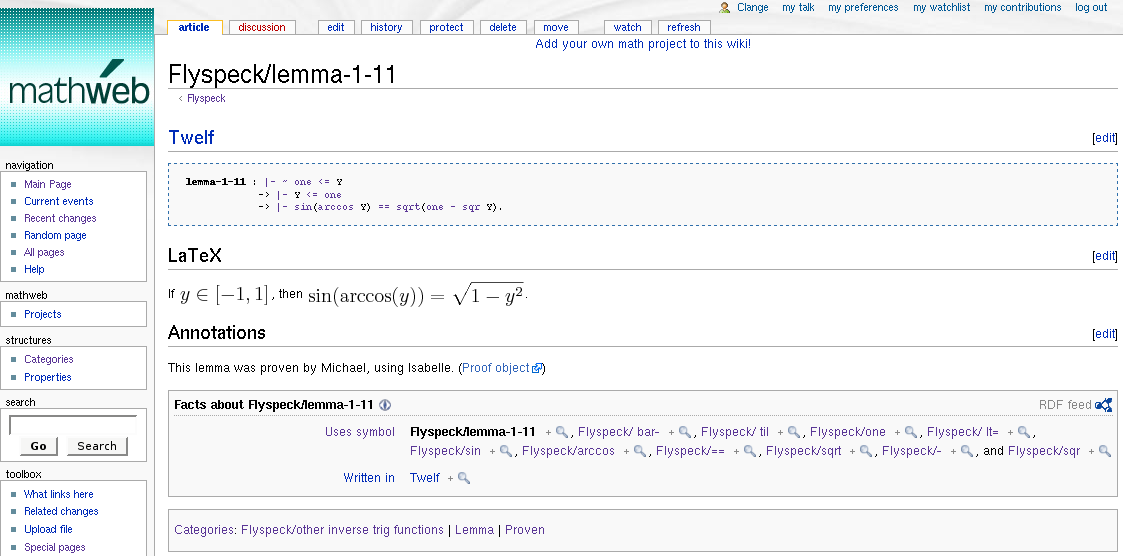
\includegraphics[width=\textwidth]{smw-lemma}
  \caption[A Flyspeck lemma in Semantic MediaWiki]{A Flyspeck lemma in Semantic
    MediaWiki\protect\footnotemark}
  \label{fig:smw-lemma}
\end{figure}
\addtocounter{footnote}{-1}
\stepcounter{footnote}\footnotetext{See \url{http://mathweb.org/wiki/Flyspeck}}

The annotations generated that way can be used for browsing, either via the summary of all
typed links in the ``fact box'', or by the special ``browse'' page.  For querying,
Semantic MediaWiki offers a simple triple search, as well as inline queries.  The latter
are intuitive to write but less powerful than SPARQL queries on an RDF store using an
OWL-DL reasoner; the query language corresponds to the description logic
$\mathcal{EL}^{++}$~\cite{KrSchVr:semwiki-reasoning07}, which, for example, does not
support negation.  A query for proven lemmas about a certain topic that have a Twelf
representation would be written as follows:

\begin{lstlisting}
<ask>[[Category:Proven]] [[Category:Lemma]]
     [[Category:Trigonometry]] [[written in::Twelf]]</ask>
\end{lstlisting}

Here, most annotations are modelled by categorization, i.\,e.\ instantiation of
classes---certainly not the most formal way of structuring knowledge in view of many
classes just corresponding to narrative sections of the book, but the one that is
supported best by Semantic MediaWiki.  More complex reasoning tasks like inference of
dependencies are not possible in Semantic MediaWiki; in this domain-specific setting one
could realize them by hard-coded extension functions.

Exporting formal representations of knowledge items is not yet supported conveniently.
The Twelf listings can be viewed on their own pages, but due to the auto-generated symbol
links in the source code, these are not suitable for download.  One would either have to
implement a special Twelf download page that cleans these sources again, or one would have
to implement the symbol linking as an extension of the rendering process.

\subsection{Towards Full Flyspeck Support in SWiM}
\label{sec:flyspeck-swim}

The experiments with Semantic MediaWiki and SWiM led to the conclusion to integrate
further support for Flyspeck in SWiM, using its rich semantic web and OMDoc
infrastructure.  Features that rely on \emph{structures}, like the linking of symbols,
could only be realized in a very prototypical way for the text-based page format of
MediaWiki, using regular expressions.  Relying on the XML infrastructure of OMDoc, these
features are easier to develop, or already available.  However, rapidly \emph{prototyping}
our first ideas about the wiki support required for Flyspeck was easier in Semantic
MediaWiki due to its ability to design ad-hoc ontologies and its implementation in the
interpreted language PHP.

use OMDoc as universal exchange format between ATP languages; every ATP system so far is
an island; OMDoc makes ATP scale to the web.  At least definitions.  However, we're not
yet sure\ednote{@Florian: right?}, whether we can actually rely on OMDoc, as translation
of \emph{proofs} is not that trivial.\ednote{@Sean/Florian: why?}

\ednote{@Florian: Would your work about theory translation somehow help?}

\ednote{@Christoph: Needs to support both preloaded and ad-hoc ontologies: The OMDoc
  document ontology is preloaded, while other annotations can be added at will. (Make SWiM
  more ``wiki''!)}

\begin{todo}{@Christoph: Elaborate on this discussion with Florian}
  OMDoc is agnostic towards logics -- that could be a benefit as long as we do not yet
  have a proof object. Work in progress, nodes without content, loosely coupled: Ideal
  setting for a wiki!  Wiki as a means of information for the collaborators about the
  progress of the \emph{whole} project.  Make a proof that's \emph{so} complex
  comprehensible in some way, show open issues/problems to potential collaborators.
  There's a whole book containing the informal outline of the proof; link the wiki to the
  book.  Probably also import the book via sTeX to the wiki.\\
  Make the whole project publicly viewable (e.g. for a progress report), make it
  manageable.\\
  Analogy: from software documentation to literate programming
\end{todo}

\ednote{@Christoph: narrative structure: do not use ad-hoc categories, but OMDoc's native
  NarCons~\cite{KohMueMue:dfncimk07}; need to be added to document ontology.}

\issue{@Florian, do you think we could make use of MathWebSearch for certain services?
  (@Sean, that's our semantic math formula search engine.)  Now that I've mentioned the
  Pythagoras example, we could think about it. --CL}

\section{Related Work (all)}
\label{sec:related}

\ednote{Again, I'll concentrate on wiki-like collaborative systems.  Is there any related
  work from the pure theorem-proving point of view?  Is there any proof comparable to
  Kepler's? --CL}

\subsection{Wikis with Integrated Proof Assistants}
\label{sec:wiki-pa}

Recently, there is a growing interest in integrating automated theorem provers or proof
assistants with wikis\footnote{See \url{http://homepages.inf.ed.ac.uk/da/mathwiki/} for
  relevant activities.}.  Both Logiweb and ProofWiki are wiki-like systems that support
checking or interactive development of proofs.  Both systems are ``semantic'' in the sense
that the integrated proof checker can utilize the mathematical knowledge in the wiki
pages.  On the other hand, the semantics is not utilized for purposes other than that,
such as facilitating browsing or editing, or connecting to services on the semantic
web.  

Developing and verifying formal proofs in the wiki is not yet the focus of Flyspeck in
this early stage, but it may be required later if the central maintainer approach does not
turn out to work.

\paragraph{Logiweb} is a distributed system for publishing machine checked mathematics in
high-quality PDF~\cite{Grue:Logiweb07}.  While the author does not call it a ``wiki'', it
shares part of the key wiki principles: Anybody can contribute to a Logiweb site and edit
new pages in a simple text syntax with a browser.  On the other hand, Logiweb does not
offer other features that would be essential for Flyspeck: browsing by traversing links is
supported neither in the editor nor in the generated PDF, and Logiweb does not offer a
built-in search or query facility.  Logiweb does not allow for \emph{exchanging} knowledge
as required for Flyspeck: Documents can be exported in presentational formats like PDF or
\TeX{}, and their internal, low-level data structures can be exported as XML or Lisp
S-expressions, but currently there is no easy way to convert these representations to
other languages for mathematical markup or theorem proving.  Finally, the way Logiweb
checks proofs is not compatible with other theorem provers, as all calculi and proof
tactics need to be defined in the Logiweb system itself.

\paragraph{ProofWiki} is an integration of ProofWeb, a web frontend to the Coq proof
assistant, into MediaWiki~\cite{CorKal:CoopReposFormalProofs07}.  Coq's converting tools
are generate human-readable and browsable HTML or {\LaTeX} presentation from the proof
scripts.  In the HTML generated that way, symbols are linked to their declaration.  Index
pages, such as lists of all definitions or all theorems, are generated, but their
generation cannot be influenced or customized through the wiki
interface\ednote{@Christoph: check!}.  So far, there is just text search, and dependencies
among knowledge items are only computed for exporting proof scripts but not used for
browsing inside the system.  Another disadvantage of ProofWiki in the context of Flyspeck
is that pages can either be formal proof scripts (with restricted possibilities to include
informal comments), or informal wiki pages.  Semi-formal documents or stepwise formalizing
of knowledge is not supported.  Importing and exporting Coq proof scripts to and from the
wiki is possible, but other formats are not yet supported.  While the authors do provide
instructions on how to integrate other theorem provers, doing so would be a lot of work,
as there is no abstraction layer or metalanguage for exchanging or converting data.

\ednote{@Christoph: Find out whether such systems have already been used in Flyspeck-like
  scenarios, i.\,e.\ collaboratively proving something.}

\section{Conclusion}
\label{sec:conc}

\ednote{Is there anything we could already conclude? --CL}

\paragraph{Acknowledgments}
\label{sec:ack}

\begin{itemize}
\item Michael Kohlhase
\item Immanuel Normann
\item Stefan Decker
\end{itemize}

\bibliographystyle{abbrv}
% load crossrefs last when using modular bib files
\bibliography{kwarc}

% \printindex

\ednotemessage
\end{document}

% vim:tw=90:autoindent: 
%%% Local Variables: 
%%% mode: latex
%%% fill-column: 90
%%% End: 
